\documentclass[conference]{IEEEtran}
\IEEEoverridecommandlockouts

% ── Core packages ─────────────────────────────────────────────────────────────
\usepackage{cite}
\usepackage{graphicx}
\usepackage{amsmath}
\usepackage{array}
\usepackage{booktabs}
\usepackage{tabularx}
\usepackage{siunitx}
\usepackage{xcolor}
\usepackage{url}
\usepackage{tikz}
\usetikzlibrary{
  arrows.meta, positioning, shapes.geometric,
  shapes.misc, calc, fit, backgrounds, shadows
}
\usepackage{enumitem}
\usepackage{listings}
\usepackage{textcomp}
\usepackage{balance}
\usepackage[hidelinks]{hyperref}

% ── Colour palette ────────────────────────────────────────────────────────────
\definecolor{colTeal50}   {HTML}{E1F5EE}
\definecolor{colTeal600}  {HTML}{0F6E56}
\definecolor{colTeal800}  {HTML}{085041}
\definecolor{colBlue50}   {HTML}{E6F1FB}
\definecolor{colBlue600}  {HTML}{185FA5}
\definecolor{colBlue800}  {HTML}{0C447C}
\definecolor{colAmber50}  {HTML}{FAEEDA}
\definecolor{colAmber600} {HTML}{854F0B}
\definecolor{colAmber800} {HTML}{633806}
\definecolor{colPurple50} {HTML}{EEEDFE}
\definecolor{colPurple600}{HTML}{534AB7}
\definecolor{colPurple800}{HTML}{3C3489}
\definecolor{colGray50}   {HTML}{F1EFE8}
\definecolor{colGray600}  {HTML}{5F5E5A}
\definecolor{colGray800}  {HTML}{444441}
\definecolor{colGreen50}  {HTML}{EAF3DE}
\definecolor{colGreen600} {HTML}{3B6D11}
\definecolor{colGreen800} {HTML}{27500A}
\definecolor{colCoral50}  {HTML}{FAECE7}
\definecolor{colCoral600} {HTML}{993C1D}
\definecolor{colCoral800} {HTML}{712B13}

% ── TikZ block-diagram styles ─────────────────────────────────────────────────
\tikzset{
  block/.style={
    draw, rounded corners=5pt,
    minimum width=36mm, minimum height=13mm,
    align=center, inner sep=5pt,
    line width=0.5pt, font=\scriptsize\sffamily
  },
  sensor/.style  ={block, fill=colBlue50,    draw=colBlue600},
  mcu/.style     ={block, fill=colTeal50,    draw=colTeal600},
  power/.style   ={block, fill=colAmber50,   draw=colAmber600},
  wifi/.style    ={block, fill=colPurple50,  draw=colPurple600},
  backend/.style ={block, fill=colGray50,    draw=colGray600},
  webui/.style   ={block, fill=colGreen50,   draw=colGreen600},
  ml/.style      ={block, fill=colCoral50,   draw=colCoral600},
  mainarr/.style ={
    -{Stealth[length=2.2mm,width=1.4mm]},
    line width=0.9pt, draw=colGray600
  },
  feedarr/.style ={
    -{Stealth[length=2.0mm,width=1.3mm]},
    line width=0.75pt, draw=colGray600,
    dashed, dash pattern=on 4pt off 3pt
  },
  % Flow-diagram node styles (for firmware / pipeline figures)
  fnode/.style={
    draw, rounded corners=4pt, align=center,
    text width=0.85\linewidth, minimum height=6.5mm,
    fill=colGray50, draw=colGray600, font=\scriptsize\sffamily
  },
  fbranch/.style={
    draw, rounded corners=4pt, align=center,
    text width=0.40\linewidth, minimum height=6.5mm,
    fill=colGray50, draw=colGray600, font=\scriptsize\sffamily
  },
  fdec/.style={
    draw, diamond, aspect=2.4, align=center,
    fill=colAmber50, draw=colAmber600,
    inner sep=1pt, font=\scriptsize\sffamily,
    minimum width=0.30\linewidth, minimum height=7.6mm
  },
  farr/.style={
    -{Stealth[length=2mm,width=1.2mm]},
    line width=0.6pt, draw=colGray600,
    shorten <=2pt, shorten >=2pt
  }
}

% ── Two-line node label ───────────────────────────────────────────────────────
\newcommand{\nodetext}[4]{%
  {\color{#1}\textbf{#2}}\\[1.5pt]%
  {\color{#3}\scriptsize #4}%
}

% ── Frame helpers ─────────────────────────────────────────────────────────────
\newcommand{\FrameBoxCol}[1]{%
  \begingroup
    \setlength{\fboxsep}{2pt}\setlength{\fboxrule}{0.4pt}%
    \fbox{\begin{minipage}{\dimexpr\columnwidth-2\fboxsep-2\fboxrule\relax}%
      \centering #1\end{minipage}}%
  \endgroup}

\newcommand{\FrameBoxText}[1]{%
  \begingroup
    \setlength{\fboxsep}{2pt}\setlength{\fboxrule}{0.4pt}%
    \fbox{\begin{minipage}{\dimexpr\textwidth-2\fboxsep-2\fboxrule\relax}%
      \centering #1\end{minipage}}%
  \endgroup}

% ── Hyperref cross-ref helpers ────────────────────────────────────────────────
\newcommand{\FigLink}[1]{\hyperref[#1]{Fig.~\ref*{#1}}}
\newcommand{\TabLink}[1]{\hyperref[#1]{Table~\ref*{#1}}}

% ── Listings ──────────────────────────────────────────────────────────────────
\lstdefinestyle{sslgcode}{
  basicstyle=\ttfamily\footnotesize,
  columns=fullflexible, keepspaces=true, breaklines=true,
  frame=single, framerule=0.3pt, rulecolor=\color{black},
  showstringspaces=false
}
\renewcommand{\IEEEkeywordsname}{Keywords}

% ── Project metadata ──────────────────────────────────────────────────────────
\newcommand{\SystemName}{Smart Sign Language Gloves: A Real-Time ISL-to-Speech Translation System}
\newcommand{\SystemAcronym}{SSLG }
\newcommand{\InstituteName}{Vidyavardhini's College Of Engineering \& Technology, Vasai Road}
\newcommand{\DeptName}{Department of Electronics and Telecommunication Engineering}
\newcommand{\TeamMemberA}{Kushagra Naresh Joshi}
\newcommand{\TeamMemberB}{Afroz Abdul Inamdar}
\newcommand{\TeamMemberC}{Sakshi Rajendra Jagdale}
\newcommand{\TeamMemberD}{Ramzan Badruduja Khan}
\newcommand{\GuideName}{Ms.\ Shaista Khan}
\newcommand{\SubmissionDate}{March 2026}
\newcommand{\TeamMemberAemail}{kushagra.2400231101@vcet.edu.in}
\newcommand{\TeamMemberBemail}{afroz.2400181201@vcet.edu.in}
\newcommand{\TeamMemberCemail}{sakshi.2400201209@vcet.edu.in}
\newcommand{\TeamMemberDemail}{ramzan.2400251108@vcet.edu.in}
\newcommand{\GuideNameemail}{shaista.khan@vcet.edu.in}
\newcommand{\CodeRepoUrl}{https://github.com/RamzanKhansLab/smart-sign-interpreter}

\title{Smart Sign Language Gloves: A Real-Time\\ISL-to-Speech Translation System}
\author{%
  \parbox{\textwidth}{\centering
    {\large\bfseries\GuideName}\\
    Assistant Professor\\
    \DeptName\\ \InstituteName\\
    Email: \GuideNameemail\\[0.5cm]
    \begin{tabular}{@{}>{\centering\arraybackslash}p{0.48\textwidth}@{\hfill}
                        >{\centering\arraybackslash}p{0.48\textwidth}@{}}
      {\large\bfseries\TeamMemberA} & {\large\bfseries\TeamMemberB}\\
      \DeptName & \DeptName\\ \InstituteName & \InstituteName\\
      Email: \TeamMemberAemail & Email: \TeamMemberBemail\\[0.5cm]
      {\large\bfseries\TeamMemberC} & {\large\bfseries\TeamMemberD}\\
      \DeptName & \DeptName\\ \InstituteName & \InstituteName\\
      Email: \TeamMemberCemail & Email: \TeamMemberDemail\\
    \end{tabular}
  }%
}

% ══════════════════════════════════════════════════════════════════════════════
\begin{document}
% ── Title page ────────────────────────────────────────────────────────────────
\begin{titlepage}
  \thispagestyle{empty}\centering\vspace*{0.8in}
  \IfFileExists{vect.png}{
\includegraphics[width=0.22\textwidth]{vect.png}\par}{}
  \vspace{0.15in}
  {\Large\textbf{\InstituteName}\par}\vspace{0.08in}
  {\large\textbf{\DeptName}\par}\vspace{0.35in}
  {\Large\textbf{\SystemName}\par}\vspace{0.2in}
  {\large\textbf{Project Guide}\par}\vspace{0.05in}
  {\large\textbf{\GuideName}\par}\vspace{0.2in}
  {\large\textbf{Team Members}\par}\vspace{0.1in}
  {\large\TeamMemberA\par}{\large\TeamMemberB\par}
  {\large\TeamMemberC\par}{\large\TeamMemberD\par}
  \vfill{\large\SubmissionDate\par}
\end{titlepage}
\clearpage\thispagestyle{empty}\null\newpage
\pagenumbering{arabic}\setcounter{page}{1}
\maketitle

% ── Abstract ──────────────────────────────────────────────────────────────────
\begin{abstract}
Indian Sign Language (ISL) remains inaccessible to most non-signers, creating
persistent communication barriers in everyday settings. This paper presents the
\textit{\SystemName} (\SystemAcronym), a wearable ISL-to-speech translation
system that delivers real-time text and spoken output directly from hand gestures.
The system employs Hall-effect sensing with fingertip magnets and a six-axis
inertial measurement unit (IMU), both interfaced to an ATmega328P microcontroller
for signal acquisition and packet framing. Sensor frames are transmitted over
Wi-Fi to a backend server that performs dataset management, model training, and
inference, with results visualised through a web-based interface. Experimental
evaluation across 20 ISL gestures yields 82--90\,\% classification accuracy
with an end-to-end latency of 220--320\,ms, confirming the feasibility of a
low-cost, portable ISL communication solution with a scalable improvement
pathway through continuous data collection.
\end{abstract}

\begin{IEEEkeywords}
assistive technology, gesture classification, Indian Sign Language~(ISL),
real-time translation, sign language recognition, wearable sensor glove
\end{IEEEkeywords}

% ══════════════════════════════════════════════════════════════════════════════
\section{Introduction}
% ══════════════════════════════════════════════════════════════════════════════

Communication barriers between hearing-impaired individuals and the general
population remain a significant societal challenge. People who rely on sign
language for daily interaction face persistent difficulties because most
listeners have no knowledge of ISL. A practical ISL translator must be
portable, low-cost, and capable of real-time response. Camera-based systems
achieve competitive recognition rates but are sensitive to lighting, framing,
and occlusion~\cite{mitra}. Wearable glove systems avoid many of these
environmental constraints; however, traditional flex-sensor designs suffer from
non-linear output drift and mechanical degradation with repeated bending.

This paper presents \SystemAcronym, a glove-based ISL translation system that
uses Hall-effect sensing combined with a backend CNN--LSTM inference pipeline to
convert multi-channel sensor patterns into ISL labels, displayed and spoken in
real time.

\subsection{Problem Formulation and Scope}

\SystemAcronym targets both camera and flex-sensor limitations through
Hall-effect sensing and a structured calibration workflow that compensates for
inter-session magnet-placement variability. The scope of this work covers:
\begin{itemize}[noitemsep, topsep=2pt]
  \item recognition of 20 commonly used ISL gestures;
  \item indoor laboratory testing under controlled conditions; and
  \item adult volunteer participants with repeatable sensor placement.
\end{itemize}

\subsection{Key Contributions}
\begin{itemize}[noitemsep, topsep=2pt]
  \item A wearable, Hall-effect-based ISL glove with integrated IMU sensing.
  \item A backend-driven training and inference pipeline enabling scalable model updates.
  \item A real-time end-to-end communication framework achieving sub-350\,ms average latency.
\end{itemize}

% ══════════════════════════════════════════════════════════════════════════════
\section{Related Work}
% ══════════════════════════════════════════════════════════════════════════════

\subsection{Vision-Based Systems}

Camera-based approaches exploit rich spatial features without requiring wearable
hardware but frequently fail under non-standard lighting, partial occlusion, or
constrained framing, and demand substantial computational resources~\cite{mitra}.

\subsection{Sensor-Based Glove Systems}

Sensor gloves measure finger and hand motion directly and operate in diverse
environments. Earlier flex-sensor designs suffer from non-linear drift and
mechanical degradation. Hall-effect sensing avoids direct mechanical contact,
yielding more stable long-term readings when magnet placement is consistent.

\subsection{Identified Gaps}

Published prototypes seldom address practical deployment concerns such as
calibration time, long-term sensor drift, wireless packet loss, or the labelling
effort needed for incremental improvement. \SystemAcronym directly targets these
gaps through a structured calibration routine, a clear labelling workflow, and
a retryable Wi-Fi transport layer.

% ══════════════════════════════════════════════════════════════════════════════
\section{Proposed Methodology}
\label{sec:methodology}
% ══════════════════════════════════════════════════════════════════════════════

\SystemAcronym is structured around two cooperating layers:
\textbf{(i)}~a \emph{glove-side sensing and sampling layer} that acquires and
frames gesture and IMU signals, and
\textbf{(ii)}~a \emph{backend software layer} that handles inference, dataset
management, and web-based visualisation.
The complete end-to-end pipeline is shown in \FigLink{fig:block}.
Each hardware component is described below with a functional summary followed
by a concise specification table.

% ─── FIGURE 1 — Full-width, half-page block diagram ──────────────────────────
\begin{figure*}[!t]
  \centering
  \FrameBoxText{%
    \begin{minipage}{0.96\linewidth}
      \centering
      \vspace{7pt}
      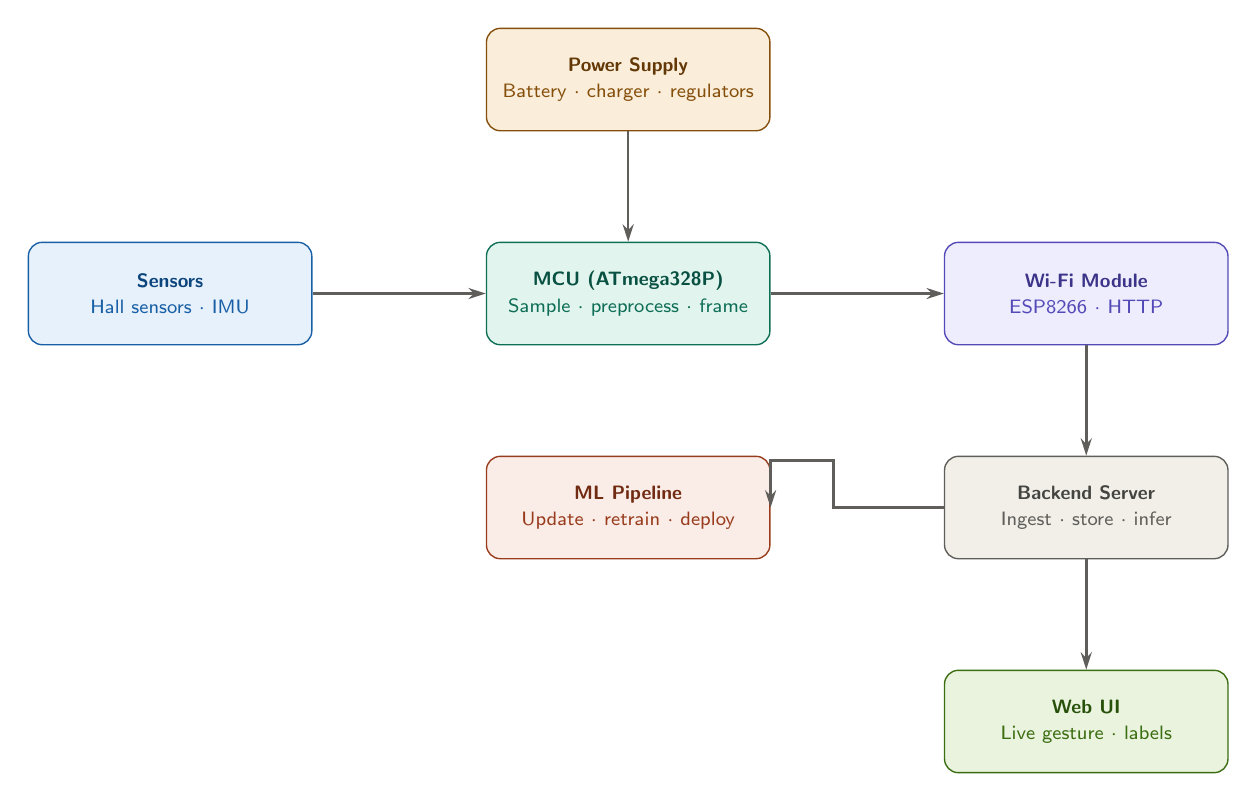
\begin{tikzpicture}[
          node distance = 14mm and 22mm,
          every node/.style={font=\scriptsize\sffamily}
      ]
        %% ── Row 1 (centre): Sensors → MCU → Wi-Fi ──────────────────────
        \node[sensor] (sens) {%
          \nodetext{colBlue800}{Sensors}{colBlue600}{Hall sensors $\cdot$ IMU}};

        \node[mcu, right=22mm of sens] (mcu) {%
          \nodetext{colTeal800}{MCU (ATmega328P)}{colTeal600}{Sample $\cdot$ preprocess $\cdot$ frame}};

        \node[wifi, right=22mm of mcu] (wifi) {%
          \nodetext{colPurple800}{Wi-Fi Module}{colPurple600}{ESP8266 $\cdot$ HTTP}};

        %% ── Row 0 (above MCU): Power ────────────────────────────────────
        \node[power, above=14mm of mcu] (pwr) {%
          \nodetext{colAmber800}{Power Supply}{colAmber600}{Battery $\cdot$ charger $\cdot$ regulators}};

        %% ── Column 3 (below Wi-Fi): Backend then Web UI ─────────────────
        \node[backend, below=14mm of wifi] (backend) {%
          \nodetext{colGray800}{Backend Server}{colGray600}{Ingest $\cdot$ store $\cdot$ infer}};

        \node[webui, below=14mm of backend] (webui) {%
          \nodetext{colGreen800}{Web UI}{colGreen600}{Live gesture $\cdot$ labels}};

        %% ── Column 2 (below MCU): ML ────────────────────────────────────
        \node[ml, below=14mm of mcu] (ml) {%
          \nodetext{colCoral800}{ML Pipeline}{colCoral600}{Update $\cdot$ retrain $\cdot$ deploy}};

        %% ── Main signal arrows ───────────────────────────────────────────
        \draw[mainarr] (sens.east) -- (mcu.west);
        \draw[mainarr] (pwr.south) -- (mcu.north);
        \draw[mainarr] (mcu.east) -- (wifi.west);
        \draw[mainarr] (wifi.south) -- (backend.north);
        \draw[mainarr] (backend.south) -- (webui.north);

        % Backend → ML (routed to avoid overlaps and keep the connection clear)
        \draw[mainarr]
          (backend.west)
          -- ++(-14mm,0)
          |- ($(ml.east)+(0,6mm)$)
          -- (ml.east);

      \end{tikzpicture}
      \vspace{7pt}
    \end{minipage}%
  }%
  \caption{%
    End-to-end system architecture of \SystemAcronym.
%
  }
  \label{fig:block}
\end{figure*}
% ─────────────────────────────────────────────────────────────────────────────

\subsection{Microcontroller — ATmega328P}

The ATmega328P is the central controller of the glove. Its 10-bit ADC samples
five Hall-effect sensor channels at a stable rate, while its
I\textsuperscript{2}C bus reads the IMU. After baseline subtraction and
lightweight filtering, it frames a UART packet and dispatches it to the
wireless module~\cite{atmega328p}. Key specifications are in
\TabLink{tab:atmega_specs}.

\begin{table}[!t]
  \centering\caption{ATmega328P key specifications}\label{tab:atmega_specs}
  \begin{tabularx}{\columnwidth}{@{}lX@{}}
    \toprule Parameter & Specification \\\midrule
    Architecture          & 8-bit AVR \\
    Max.\ clock           & 20\,MHz \\
    Flash / SRAM / EEPROM & 32\,KB / 2\,KB / 1\,KB \\
    Supply voltage        & 1.8\,V -- 5.5\,V \\
    GPIO                  & 23 programmable I/O \\
    ADC                   & 10-bit, up to 8 channels \\
    Interfaces            & USART, SPI, I\textsuperscript{2}C (TWI) \\
    Operating temp.       & $-40$\textdegree C to $+85$\textdegree C \\
    \bottomrule
  \end{tabularx}
\end{table}

\subsection{Gesture Sensors — SS49E Hall-Effect}

Small neodymium magnets affixed to each fingertip alter the magnet-to-sensor
distance when a finger bends, producing a characteristic multi-channel analog
signature. Hall-effect sensing is preferred over flex sensors for its
durability and repeatability; residual inter-session variability is handled
by the calibration routine described in Section~\ref{sec:calib}~\cite{ss49e}.

\begin{table}[!t]
  \centering\caption{SS49E Hall-effect sensor key specifications}\label{tab:hall_specs}
  \begin{tabularx}{\columnwidth}{@{}lX@{}}
    \toprule Parameter & Specification \\\midrule
    Supply voltage  & 3\,V -- 6\,V \\
    Output type     & Analog ratiometric \\
    Sensitivity     & $\approx$1--2\,mV/Gauss \\
    Response time   & 2\,\textmu s (typ.) \\
    Operating temp. & $-40$\textdegree C to $+85$\textdegree C \\
    Package         & TO-92 \\
    \bottomrule
  \end{tabularx}
\end{table}

\subsection{Inertial Measurement Unit — MPU-6050}

The IMU provides three-axis acceleration and three-axis angular-rate data to
capture wrist and hand-orientation context. This additional channel resolves
ambiguous gestures that share similar finger configurations but differ in hand
orientation~\cite{mpu6050}.

\begin{table}[!t]
  \centering\caption{MPU-6050 IMU key specifications}\label{tab:mpu_specs}
  \begin{tabularx}{\columnwidth}{@{}lX@{}}
    \toprule Parameter & Specification \\\midrule
    Supply voltage   & 2.375\,V -- 3.46\,V \\
    Gyro full-scale  & $\pm$250 / 500 / 1000 / 2000\,\textdegree/s \\
    Accel full-scale & $\pm$2 / 4 / 8 / 16\,g \\
    ADC resolution   & 16-bit \\
    Interface        & I\textsuperscript{2}C (up to 400\,kHz) \\
    FIFO buffer      & 1024\,bytes \\
    Operating temp.  & $-40$\textdegree C to $+85$\textdegree C \\
    \bottomrule
  \end{tabularx}
\end{table}

\subsection{Wi-Fi Module — ESP8266}

The ESP8266 bridges the UART stream from the MCU to the backend server over
IEEE\,802.11\,b/g/n using HTTP POST requests. A dedicated switching 3.3\,V
rail (separate from the USB adapter) supplies the module to handle peak
transmit bursts without brownout~\cite{esp8266}.

\begin{table}[!t]
  \centering\caption{ESP8266 Wi-Fi module key specifications}\label{tab:esp_specs}
  \begin{tabularx}{\columnwidth}{@{}lX@{}}
    \toprule Parameter & Specification \\\midrule
    Supply voltage  & 3.0\,V -- 3.6\,V (3.3\,V nom.) \\
    Wi-Fi standard  & IEEE 802.11 b/g/n (2.4\,GHz) \\
    Peak TX current & $\approx$215\,mA (burst) \\
    Modes           & Station / Soft-AP / Station+AP \\
    UART rate       & 115200\,bps (AT firmware, default) \\
    Security        & WPA/WPA2-Personal \\
    Operating temp. & $-40$\textdegree C to $+125$\textdegree C \\
    \bottomrule
  \end{tabularx}
\end{table}

\subsection{Power Sub-System}

Three modules manage the power chain:
\begin{itemize}[noitemsep, topsep=2pt]
  \item \textbf{Li-ion cell} (3.6\,V nominal, 1800--3500\,mAh) — primary
        energy source with over-charge, over-discharge, and short-circuit
        protection~\cite{battery18650}.
  \item \textbf{TP4056 charger} — CC/CV linear charger supplying up to
        1000\,mA from a 5\,V USB input with 4.2\,V regulation~\cite{tp4056}.
  \item \textbf{MT3608 boost + LM2596 buck} — step-up to 5\,V for the
        MCU and sensor front-end; step-down to 3.3\,V for the
        Wi-Fi module~\cite{mt3608,lm2596}.
\end{itemize}

\begin{table}[!t]
  \centering\caption{Power sub-system key specifications}\label{tab:power_specs}
  \begin{tabularx}{\columnwidth}{@{}llX@{}}
    \toprule Module & Parameter & Value \\\midrule
    Li-ion cell  & Nom.\ / full-charge voltage & 3.6\,V / 4.2\,V \\
                 & Capacity                    & 1800--3500\,mAh \\
    TP4056       & Charge current (max)        & 1000\,mA \\
                 & Termination current         & $0.1\times I_\text{CHG}$ \\
    MT3608 boost & $V_\text{OUT}$              & 5\,V (adjustable) \\
                 & Peak efficiency             & up to 93\,\% \\
    LM2596 buck  & $V_\text{OUT}$              & 3.3\,V (adjustable) \\
                 & Rated output current        & 3\,A \\
    \bottomrule
  \end{tabularx}
\end{table}

\subsection{USB-to-UART Adapter}

An FTDI-compatible USB-to-UART adapter is used for firmware flashing and
serial debug during development only. The Wi-Fi module is powered from the
on-board 3.3\,V regulated rail during flashing to avoid overloading the
adapter's limited regulator~\cite{ft232rl}.

\subsection{Communication Protocol and Packet Format}

The MCU transmits sensor frames to the ESP8266 over UART at 115200\,bps.
The ESP8266 forwards each frame to the backend via HTTP POST. HTTP status
codes provide a lightweight acknowledgment mechanism for detecting packet loss.
The 28-byte frame structure is detailed in \TabLink{tab:packet}.

\begin{table}[!t]
  \centering\caption{UART packet format (MCU to Wi-Fi module)}\label{tab:packet}
  \begin{tabularx}{\columnwidth}{@{}lcX@{}}
    \toprule Field & Bytes & Description \\\midrule
    Preamble       & 1  & 0xAA sync byte \\
    Version        & 1  & Protocol version \\
    Timestamp      & 2  & Milliseconds mod 65536 \\
    Gesture[0--4]  & 10 & 5 channels, 2\,bytes each (ADC) \\
    IMU[0--5]      & 12 & 6 axes, 2\,bytes each \\
    Label ID       & 1  & Optional during collection mode \\
    Checksum       & 1  & XOR of all payload bytes \\
    \midrule
    \textbf{Total} & \textbf{28} & \\
    \bottomrule
  \end{tabularx}
\end{table}

\subsection{Calibration Procedure}
\label{sec:calib}

Before each session, the user holds a neutral open-palm pose for 3\,s. The
firmware computes a per-channel baseline $b_i$ (mean over the window) and
stores it in EEPROM. All subsequent readings use the relative deflection
\begin{equation}
  \Delta_i \;=\; x_i - b_i ,
  \label{eq:calib}
\end{equation}
ensuring the classifier learns pose-relative patterns rather than absolute
ADC levels. An equivalent bias-subtraction step is applied to the accelerometer
channels to remove static gravity bias.

\subsection{Windowing and Feature Formation}

The sensor stream is segmented into overlapping windows of $W$ samples
(e.g., 25--50) with 50\,\% overlap. Each window forms a tensor of shape
$W \times C$, where $C = 11$ (5 Hall-effect channels $+$ 6 IMU channels).
This format is directly compatible with 1-D convolutional and recurrent layers
and reduces sensitivity to small timing differences between signers.

\subsection{Model Architecture and Training Pipeline}

A CNN--LSTM architecture captures both local temporal features and long-range
sequential dependencies:
\begin{itemize}[noitemsep, topsep=2pt]
  \item \textbf{Feature extraction:} two 1-D convolutional layers
        (kernel size~3; 32 and 64 filters) with ReLU activations.
  \item \textbf{Temporal encoding:} one LSTM layer with 128 units.
  \item \textbf{Output head:} dense softmax over 20 gesture classes.
\end{itemize}
Dropout (rate 0.4) mitigates overfitting; AMSGrad minimises categorical
cross-entropy. The trained model is quantised to 8-bit precision for
low-latency deployment. The training workflow is visualised in
\FigLink{fig:mlflow}.

\begin{figure}[htbp]
  \centering
  \FrameBoxCol{%
    \begin{minipage}{0.94\linewidth}\centering
      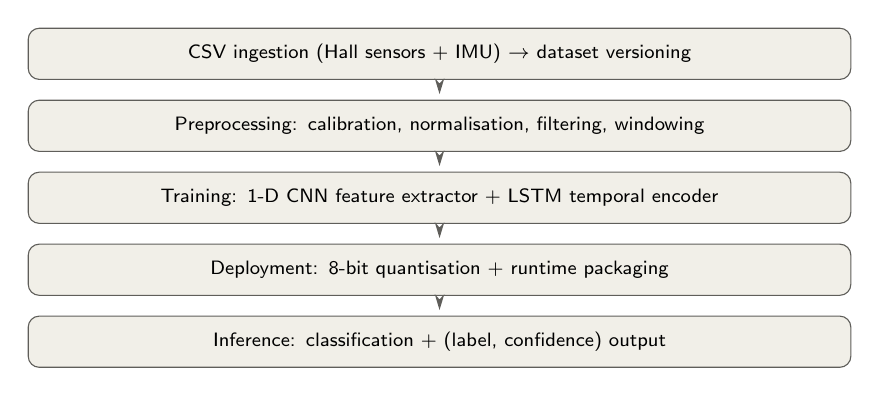
\begin{tikzpicture}[font=\scriptsize, node distance=2.5mm,
                          every node/.style={inner sep=2pt}]
        \node[fnode] (ing)  {CSV ingestion (Hall sensors + IMU) $\rightarrow$ dataset versioning};
        \node[fnode, below=of ing]  (prep) {Preprocessing: calibration, normalisation, filtering, windowing};
        \node[fnode, below=of prep] (train){Training: 1-D CNN feature extractor + LSTM temporal encoder};
        \node[fnode, below=of train](tfl)  {Deployment: 8-bit quantisation + runtime packaging};
        \node[fnode, below=of tfl]  (inf)  {Inference: classification + (label, confidence) output};
        \draw[farr](ing)--(prep); \draw[farr](prep)--(train);
        \draw[farr](train)--(tfl); \draw[farr](tfl)--(inf);
      \end{tikzpicture}
    \end{minipage}}%
  \caption{High-level model training and inference workflow for \SystemAcronym.}
  \label{fig:mlflow}
\end{figure}

\subsection{Firmware Processing Flow}

\begin{figure}[htbp]
  \centering
  \FrameBoxCol{%
    \begin{minipage}{0.94\linewidth}\centering
      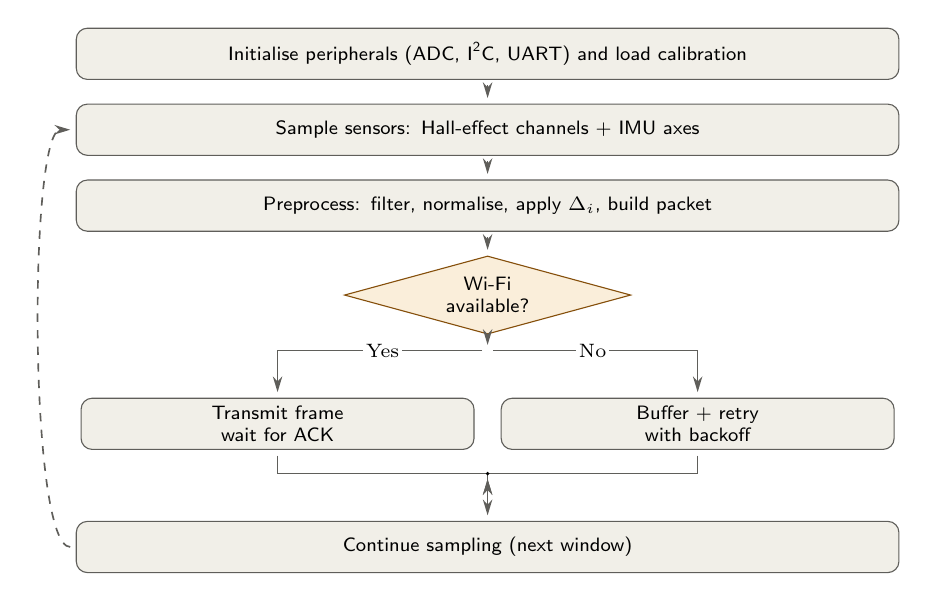
\begin{tikzpicture}[font=\scriptsize, every node/.style={inner sep=2pt}]
        \node[fnode] (init)   {Initialise peripherals (ADC, I\textsuperscript{2}C, UART) and load calibration};
        \node[fnode, below=3mm of init]   (sample){Sample sensors: Hall-effect channels + IMU axes};
        \node[fnode, below=3mm of sample] (prep)  {Preprocess: filter, normalise, apply $\Delta_i$, build packet};
        \node[fdec,  below=3mm of prep]   (wifiok){Wi-Fi\\available?};
        \node[fbranch, below=8mm of wifiok, xshift=-0.22\linewidth] (tx)  {Transmit frame\\wait for ACK};
        \node[fbranch, below=8mm of wifiok, xshift= 0.22\linewidth] (buf) {Buffer + retry\\with backoff};
        \coordinate (merge) at ($(tx.south)!0.5!(buf.south)+(0,-3mm)$);
        \node[fnode, below=6mm of merge] (next) {Continue sampling (next window)};
        \draw[farr](init)--(sample); \draw[farr](sample)--(prep);
        \draw[farr](prep)--(wifiok);
        \coordinate (drop) at ($(wifiok.south)+(0,-2mm)$);
        \draw[farr](wifiok.south)--(drop);
        \draw[farr](drop) -| node[pos=0.25,fill=white,inner sep=1pt]{Yes} (tx.north);
        \draw[farr](drop) -| node[pos=0.25,fill=white,inner sep=1pt]{No}  (buf.north);
        \draw[farr](tx.south)  -- ++(0,-3mm) -| (merge);
        \draw[farr](buf.south) -- ++(0,-3mm) -| (merge);
        \fill(merge) circle(0.7pt);
        \draw[farr](merge)--(next.north);
        \draw[farr, dashed](next.west)..controls+(-6mm,0)and+(-6mm,0)..(sample.west);
      \end{tikzpicture}
    \end{minipage}}%
  \caption{Firmware-level acquisition and transmission flow on the ATmega328P.}
  \label{fig:firmware}
\end{figure}

\subsection{Backend Architecture and Data Management}

The Flask backend~\cite{flask} operates through five sequential, independently
debuggable stages:
\begin{enumerate}[noitemsep, topsep=2pt, label=\textbf{\arabic*.}]
  \item \textbf{Ingest} — decode HTTP frames and persist raw CSV rows.
  \item \textbf{Label} — assign gesture IDs and session metadata via the web UI.
  \item \textbf{Preprocess} — calibrate, normalise, filter, and window into a
        versioned dataset.
  \item \textbf{Train} — fit the CNN--LSTM model; export evaluation logs.
  \item \textbf{Infer} — classify a new window; return label and confidence.
\end{enumerate}
The workflow is illustrated in \FigLink{fig:backendflow}. REST endpoints are:
\begin{itemize}[noitemsep, topsep=2pt]
  \item \texttt{POST /api/ingest} — receive and store decoded packets;
  \item \texttt{POST /api/label}  — confirm labels for a buffered window;
  \item \texttt{POST /api/train}  — trigger training on selected dataset version;
  \item \texttt{POST /api/infer}  — return predicted label and confidence;
  \item \texttt{GET  /ui/collect}, \texttt{/ui/label}, \texttt{/ui/infer} — Jinja2 pages.
\end{itemize}

\begin{figure}[htbp]
  \centering
  \FrameBoxCol{%
    \begin{minipage}{0.94\linewidth}\centering
      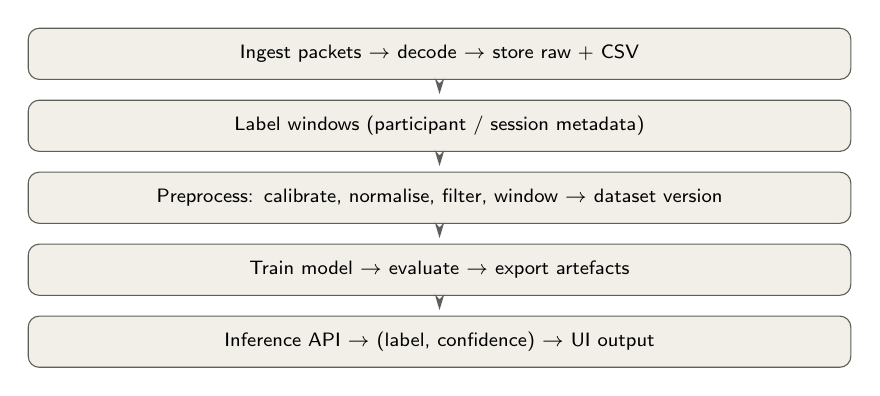
\begin{tikzpicture}[font=\scriptsize, node distance=2.5mm,
                          every node/.style={inner sep=2pt}]
        \node[fnode] (ing)  {Ingest packets $\rightarrow$ decode $\rightarrow$ store raw + CSV};
        \node[fnode, below=of ing]  (lab)  {Label windows (participant / session metadata)};
        \node[fnode, below=of lab]  (prep) {Preprocess: calibrate, normalise, filter, window $\rightarrow$ dataset version};
        \node[fnode, below=of prep] (train){Train model $\rightarrow$ evaluate $\rightarrow$ export artefacts};
        \node[fnode, below=of train](infer){Inference API $\rightarrow$ (label, confidence) $\rightarrow$ UI output};
        \draw[farr](ing)--(lab); \draw[farr](lab)--(prep);
        \draw[farr](prep)--(train); \draw[farr](train)--(infer);
      \end{tikzpicture}
    \end{minipage}}%
  \caption{Backend workflow: data collection, labelling, versioning, training, and inference.}
  \label{fig:backendflow}
\end{figure}

\subsection{Circuit Overview}

The complete schematic — covering the power tree, sensor interfaces, MCU
wiring, and Wi-Fi uplink — is shown in \FigLink{fig:circuit}.

\begin{figure*}[t]
  \centering
  \IfFileExists{KICAD_SSGL_PDF.pdf}{%
    \FrameBoxText{%
      \includegraphics[page=1,width=\linewidth,height=0.70\textheight,
        keepaspectratio,trim=40mm 85mm 40mm 80mm,clip]{KICAD_SSGL_PDF.pdf}}%
  }{%
    \IfFileExists{sslg_full_circuit.png}{%
      \FrameBoxText{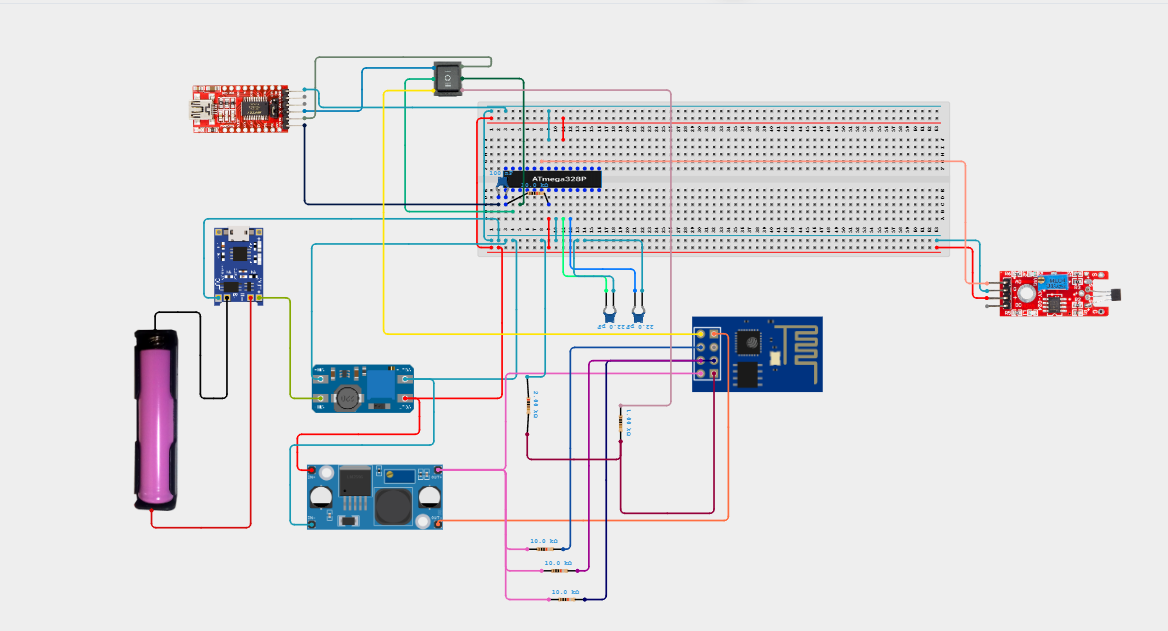
\includegraphics[width=\linewidth,keepaspectratio]{sslg_full_circuit.png}}%
    }{%
      \FrameBoxText{\parbox{0.95\linewidth}{\centering\textbf{Circuit diagram placeholder}\\
        Add \texttt{KICAD\_SSGL\_PDF.pdf} (preferred) or
        \texttt{sslg\_full\_circuit.png}.}}%
    }%
  }%
  \caption{Complete circuit schematic of \SystemAcronym{} (KiCad export).}
  \label{fig:circuit}
\end{figure*}

% ══════════════════════════════════════════════════════════════════════════════
\section{Implementation}
% ══════════════════════════════════════════════════════════════════════════════

\subsection{Source Code Repository}

All firmware, backend, and training scripts are publicly available
at~\url{\CodeRepoUrl}~\cite{githubrepo}.

\subsection{Data Collection and Preprocessing}

Volunteers perform each of the 20 ISL gestures across multiple sessions.
Each session generates labelled CSV rows stored on the backend server.
Preprocessing normalises each channel and applies a moving-average filter.
Oversampling balances under-represented classes, targeting approximately
1000 records per gesture. \TabLink{tab:dataset} summarises the structure.

\begin{table}[!t]
  \centering\caption{Dataset snapshot (representative structure)}\label{tab:dataset}
  \begin{tabularx}{\columnwidth}{@{}lrX@{}}
    \toprule Gesture & Samples & Dominant sensor signature \\\midrule
    Hello          & 1024    & Strong Hall deflection on thumb \\
    Thank you      &  980    & Subtle wrist tilt + multi-channel shift \\
    Yes            & 1012    & Flexed-finger combination \\
    No             &  995    & Accelerometer variance \\
    Others (16)    & 16\,000 & Balanced mix \\
    \bottomrule
  \end{tabularx}
\end{table}

The stored CSV follows the fixed schema in \TabLink{tab:csvschema}.

\begin{table}[!t]
  \centering\caption{CSV column schema}\label{tab:csvschema}
  \begin{tabularx}{\columnwidth}{@{}lX@{}}
    \toprule Column & Description \\\midrule
    \texttt{ts\_ms}          & Timestamp (milliseconds) \\
    \texttt{gesture0..4}     & Raw Hall-effect ADC channels (5) \\
    \texttt{ax, ay, az}      & Accelerometer axes \\
    \texttt{gx, gy, gz}      & Gyroscope axes \\
    \texttt{label\_id}       & Gesture identifier (integer) \\
    \texttt{label\_name}     & Gesture name (string) \\
    \texttt{participant\_id} & Anonymous participant ID \\
    \texttt{session\_id}     & Session identifier \\
    \bottomrule
  \end{tabularx}
\end{table}

\subsection{Power Budget Estimation}

Battery autonomy is characterised by recording: (i)~average current during
idle sensor collection, (ii)~average current during Wi-Fi inference bursts
(200--300\,mA peak), and (iii)~total runtime to the 3.0\,V cell cutoff.
This power characterisation is reported alongside accuracy and latency.

% ══════════════════════════════════════════════════════════════════════════════
\section{Results and Discussion}
% ══════════════════════════════════════════════════════════════════════════════

\subsection{Experimental Setup}

Experiments were conducted in a university laboratory using a dedicated 2.4\,GHz
access point to minimise interference. The backend ran on an Intel Core\,i5-class
laptop (8\,GB RAM). Each session began with the 3-second open-palm calibration.
Round-trip latency was logged from sensor packet capture to inference response.

\subsection{Performance Metrics}

\TabLink{tab:metrics} summarises measured classification and latency results.

\begin{table}[!t]
  \centering\caption{Measured performance metrics}\label{tab:metrics}
  \begin{tabularx}{\columnwidth}{@{}lX@{}}
    \toprule Metric & Value \\\midrule
    Accuracy (\%)                 & 82 -- 90 \\
    Precision                     & 0.87 \\
    Recall                        & 0.91 \\
    F1-score                      & 0.91 -- 0.93 \\
    Avg.\ end-to-end latency (ms) & 220 -- 320 \\
    Peak end-to-end latency (ms)  & 450 -- 650 \\
    Battery autonomy (hours)      & 3 -- 5 \\
    \bottomrule
  \end{tabularx}
\end{table}

\subsection{Comparative Analysis}

\TabLink{tab:comparison} positions \SystemAcronym against common alternatives.

\begin{table}[!t]
  \centering\caption{Qualitative comparison of gesture-recognition approaches}
  \label{tab:comparison}
  \begin{tabularx}{\columnwidth}{@{}>{\raggedright\arraybackslash}p{0.28\columnwidth}XX@{}}
    \toprule Approach & Strengths & Limitations \\\midrule
    Camera-based &
      No wearable hardware; rich features &
      Occlusion; lighting; compute cost~\cite{mitra} \\
    Flex-sensor glove &
      Low-complexity; direct bend &
      Fatigue; drift; non-linearity \\
    \SystemAcronym{} (Hall) &
      Durable; portable; low cost &
      Magnet placement; calibration \\
    \bottomrule
  \end{tabularx}
\end{table}

\subsection{Discussion}

Hall-effect sensing reduces mechanical wear compared to flex-based approaches
and provides stable readings when magnet placement is consistent. The
web-based labelling workflow streamlines iterative data collection and
retraining. The primary practical challenges are ensuring repeatable magnet
placement across users and sessions, robust calibration under real-world
conditions, and managing occasional Wi-Fi packet loss. Per-class confusion
analysis and training-curve plots are generated internally; aggregate metrics
are reported here due to space constraints.

% ══════════════════════════════════════════════════════════════════════════════
\section{Conclusion}
% ══════════════════════════════════════════════════════════════════════════════

\SystemAcronym demonstrates the feasibility of a portable, low-cost ISL
translation system. A Hall-effect sensor glove with integrated IMU feeds an
ATmega328P sampling layer, which transmits frames over Wi-Fi to a backend
CNN--LSTM inference engine that returns text and speech output. Experimental
results confirm 82--90\,\% classification accuracy at 220--320\,ms
end-to-end latency under laboratory conditions. The modular architecture
accommodates larger datasets and further latency optimisations without
hardware redesign.

% ══════════════════════════════════════════════════════════════════════════════
\section{Future Scope}
% ══════════════════════════════════════════════════════════════════════════════

Future work will focus on:
\begin{itemize}[noitemsep, topsep=2pt]
  \item expanding the gesture vocabulary and user population for broader coverage;
  \item integrating on-device inference (e.g., TensorFlow Lite~\cite{tensorflow})
        to eliminate network dependency; and
  \item improving automatic recalibration and long-term drift compensation.
\end{itemize}

\section*{Acknowledgment}

The authors thank the \DeptName, \InstituteName, for providing laboratory
facilities and guidance throughout this project.

\balance

% ── Bibliography ──────────────────────────────────────────────────────────────
\begin{thebibliography}{99}

\bibitem{mitra}
S.~Mitra and T.~Acharya,
``Gesture recognition: A survey,''
\textit{IEEE Trans.\ Syst., Man, Cybern.\ Part~C},
vol.~37, no.~3, pp.~311--324, May~2007.
[Online]. Available: \url{https://ieeexplore.ieee.org/document/4154947}

\bibitem{tensorflow}
TensorFlow Lite,
``TensorFlow Lite guide,'' 2024.
[Online]. Available: \url{https://www.tensorflow.org/guide}

\bibitem{atmega328p}
Microchip Technology,
``8-bit microcontroller datasheet,'' 2016.
[Online]. Available: \url{https://www.microchip.com/en-us/product/ATmega328P}

\bibitem{ft232rl}
FTDI, ``USB-to-UART converter IC.''
[Online]. Available: \url{https://ftdichip.com/products/ft232rl/}

\bibitem{tp4056}
``Single-cell Li-ion battery charger IC datasheet.''
[Online]. Available:
\url{https://img.eecart.com/dev/file/part/spec/TP4056-XUNDE.pdf}

\bibitem{battery18650}
``Lithium-ion cylindrical cell overview.''
[Online]. Available: \url{https://en.wikipedia.org/wiki/18650_battery}

\bibitem{mt3608}
``Boost converter IC datasheet.''
[Online]. Available:
\url{https://www.ic-components.com/blog/mt3608-step-up-converter-datasheet,pinout,and-applications.jsp}

\bibitem{lm2596}
Texas Instruments,
``Buck (step-down) power converter datasheet.''
[Online]. Available: \url{https://www.ti.com/lit/ds/symlink/lm2596.pdf}

\bibitem{esp8266}
Espressif Systems,
``Wi-Fi module datasheet,'' 2019.
[Online]. Available:
\url{https://www.espressif.com/sites/default/files/documentation/0a-esp8266ex_datasheet_en.pdf}

\bibitem{ss49e}
Honeywell,
``Linear Hall-effect sensor datasheet.''
[Online]. Available:
\url{https://www.mouser.com/datasheet/2/187/SS49E-1122400.pdf}

\bibitem{mpu6050}
TDK InvenSense,
``6-axis IMU product specification,'' 2015.
[Online]. Available:
\url{https://robu.in/wp-content/uploads/2014/12/GY-87_EN.pdf}

\bibitem{flask}
Pallets Projects,
``Flask documentation,'' 2024.
[Online]. Available: \url{https://flask.palletsprojects.com/en/2.2.x/}

\bibitem{githubrepo}
GitHub, ``\SystemName\ source code repository.''
[Online]. Available: \url{\CodeRepoUrl}

\end{thebibliography}

\end{document}
